%!TEX root=document.tex

\section{View Pruning Framework}
\label{sec:pruning_framework}
% The previous section described techniques to
% batch and share computations across queries---however,
% if the number of queries is large, this can still 
% lead to high execution times.
Although it is possible to construct hundreds of potential (aggregate)
visualizations for a typical dataset, only a fraction of these visualizations have high utility and are relevant to the user.
Most visualizations are low-utility and computational resources
are wasted in computing these visualizations.
% Moreover, only a fraction of the visualizations evaluated by
% \SeeDB are of high quality; most models have low utility and
% computational resources are wasted in computing these visualizations.
In this section, we describe \SeeDB's view pruning framework used to 
eliminate many views without completely evaluating them.

\stitle{Basic Pruning Framework.}
\label{subsec:basic_framework}
Recall that the pruning algorithm executes in phases, with each phase partially evaluating optimized query batches
on a subset of the data.
Specifically, after each phase, \SeeDB estimates the utility of each view on data from the current and previous batches, and eliminates
low-utility views that are very unlikely to be in the top-$k$.  It also can accept certain views as definitely being in the top-$k$.
If more than $k$ views remain, it iterates over the next batch of data;  otherwise the top-$k$ views are returned to the front end.
This process is shown in Algorithm~\ref{algo:custom_exec_engine}.


\begin{algorithm}[h]
\caption{Pruning Framework}
\label{algo:custom_exec_engine}
\begin{algorithmic}[1]
\State viewsInRunning $\gets$ \{all views\}
\State currPhase $\gets$ 0
\While {currPhase.hasNext()}
\State processNextPartition()
%\State updateUtilityEstimates()
\If {currPhase.End()}
\State pruneViews(viewsInRunning)
\State currPhase.Next()
\EndIf
% \If {stoppingCondition.True()}
% \State break
% \EndIf
\EndWhile
\State return viewsInRunning.sort().getTopK()
\end{algorithmic}
\end{algorithm}


We implemented two different pruning schemes in \SeeDB.
The first scheme uses  confidence-interval
techniques to bound utilities of views, while the second uses
multi-armed bandit allocation strategies to find top utility views.

\stitle{Confidence Interval-Based Pruning.}
\label{sec:confidence_interval}
This pruning scheme uses worst-case statistical confidence intervals to bound utility estimates obtained as \SeeDB
processes larger fractions of the underlying dataset.
Our pruning technique is similar to top-k based pruning 
algorithms developed 
in other contexts as described in ~\cite{DBLP:conf/pods/FaginLN01, 
DBLP:conf/vldb/IlyasAE04, DBLP:conf/ICDE/ReDS07}.

Pruning works as follows: at every point during execution, \SeeDB
maintains a running estimate of the mean utility $u_i$ for every view 
$V_i$ and a confidence interval around that mean, $u_i \pm c_i$.	

At the end of a phase, we use the estimates $u_i \pm c_i$ to prune low-utility views according to the following rule:
{\em If the upper bound of the utility of view $V_i$ is lesser
than the lower bound of the utility of $k$ or more views, then $V_i$ is discarded.}
To illustrate, suppose a dataset has four views $V_1$ to $V_4$ and we wish to find the top-$2$ views.
Further suppose that at the end of phase $p$,
$V_1$-$V_4$ have utility confidence intervals as shown in Figure \ref{fig:conf_interval}.
Views $V_1$ and $V_2$ have the highest estimates for utility so far.
Consider view $V_3$; we see that $V_3$'s confidence interval overlaps with the
confidence intervals of the current top views, making it possible
that $V_3$ will be in the final top views. On the other hand, the confidence
interval for $V_4$ lies entirely below the lowerbounds of $V_1$ and $V_2$.
Since we can claim with high probability
that the utility of $V_4$ lies within its confidence interval, it follows that
with high probability, $V_4$'s utility will be lower than that of both $V_1$ and
$V_2$, and it will not appear in the top-$2$ views.
We state the algorithm formally in
Algorithm~\ref{algo:ci_based_pruning}.

\begin{figure}[h]
\vspace{-10pt}
\centerline{
\hbox{\resizebox{8cm}{!}{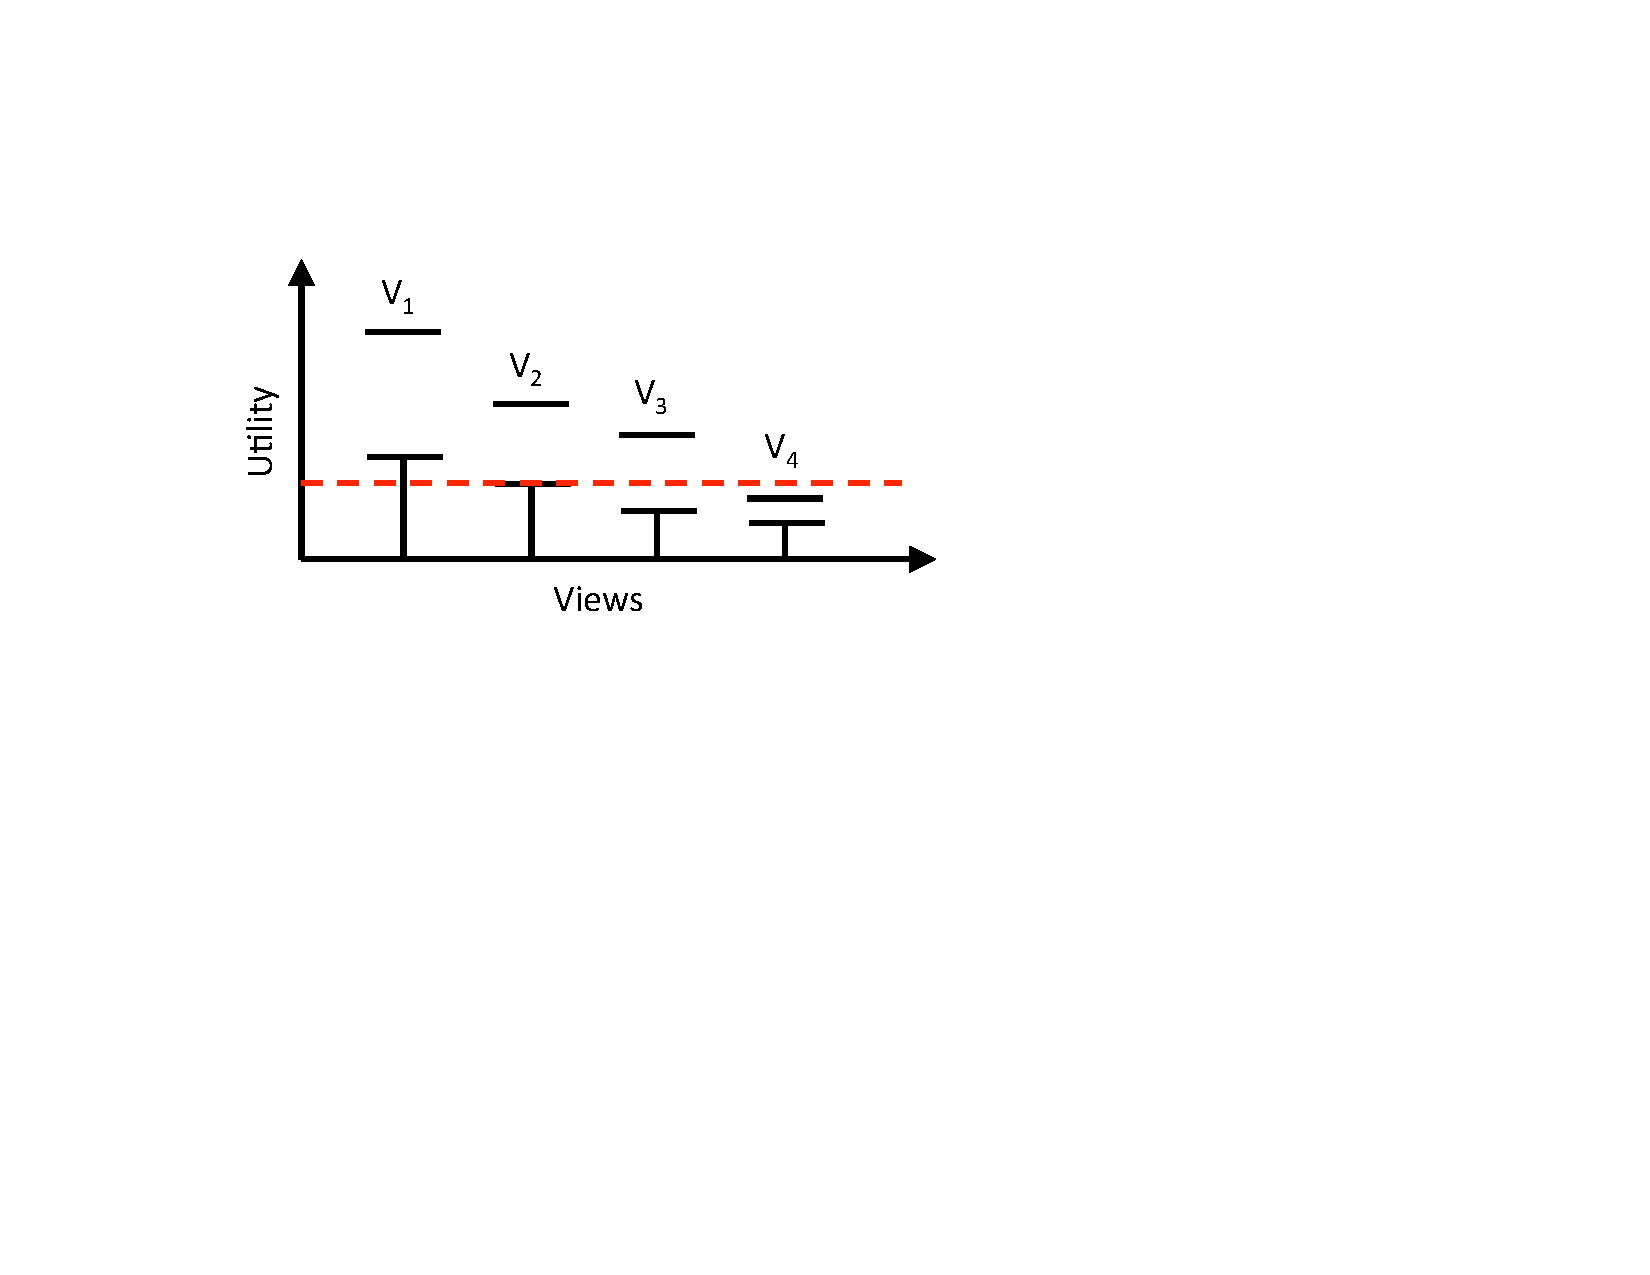
\includegraphics[trim=10mm 100mm 55mm 35mm, 
clip=true]{Images/confidence_pruning.pdf}}}}
\vspace{-20pt}
\caption{Confidence Interval based Pruning}
\label{fig:conf_interval}
\vspace{-15pt}
\end{figure}

\reviewer {
	V5 is extraneous
}


% \papertext{Pseudocode for our pruning scheme can be found in our technical report~\cite{seedb-tr}.}

\begin{algorithm}
\caption{Confidence Interval Based Pruning}
\label{algo:ci_based_pruning}
\begin{algorithmic}[1]
\State viewsInRunning.sortByUpperbound()
\State topViews $\gets$ viewsInRunning.getTopK()
\State lowestLowerbound $\gets$ min(lowerbound(topViews))
\For {view $\not \in$ topViews}
\If {view.upperbound < lowestLowerbound}
\State viewsInRunning.remove(view)
\EndIf
\EndFor
\end{algorithmic}
\end{algorithm}

To obtain conservative bounds, we use {\it worst case} confidence intervals as derived from
the Hoeffding-Serfling inequality~\cite{serfling1974probability}.
The inequality states that if we are given $N$ values $y_1, \ldots, y_N$ in 
$[0, 1]$ with average $\mu$, and we have have drawn $m$ values without replacement, $Y_1, \ldots, Y_m$, 
then we can calculate a running confidence interval around the current mean 
of the $m$ values such that the actual mean of the $N$
is always within this confidence interval with a probability of $1 - \delta$:
\begin{theorem}
\label{thm:hs}

Fix any $\delta > 0$. For $1 \le m \le N-1$, define
{\small $$
\varepsilon_m = \sqrt{\frac{(1-\frac{m-1}N)(2\log \log (m) + \log(\pi^2/3\delta))}{2m}}.
$$
$$
\textrm{Then:} \ \   \Pr\left[ \exists m, 1 \le m \le N : 
  \left|\frac{\sum_{i=1}^m Y_i}{m} - \mu\right| > \varepsilon_m \right] 
\le \delta.
$$
}

\end{theorem}
In our setting, each $Y_i$ corresponds to an estimate of utility computed based on the
records seen so far. 


\stitle{Multi-Armed Bandit Pruning.}
\label{sec:multi_armed_bandit}
%The \SeeDB pruning problem seeks to start with a large set of potential
%visualizations and to rapidly narrow them at run-time to the set of 
%visualizations with the highest utility.
Our second pruning scheme uses an adapative of a Multi-Armed Bandit (MAB)~\cite{bandits, AuerCF02, LaiR85} to identify top views.
In MAB, an online algorithm chooses from a set of alternatives (arms)
 over a sequence of trials to maximize reward.  In our setting,the  alternatives correspond to various visualizations and the reward corresponds
 to utility. 
We note that this is the first time that bandit strategies have been
applied to the problem of identifying interesting visualizations.

\techreport{The setting of MAB is as follows: a gambler is faced with several slot
machines (``one-armed bandit''s), each of which has an underlying 
(unknown) reward distribution. 
Every play results in a reward from the corresponding machine's
reward distribution.
The goal is to devise a {\it strategy} of which machine to play
at each turn in order to maximize the reward~\cite{bandits}.}
A recently-studied variation of MAB focuses on finding the arms with the highest
mean rewards~\cite{BubeckWV13, audibert2010best}.
Under certain \srm{which?} assumptions, this variation is identical to the problem addressed by \SeeDB: our goal is find the views (arms) with the 
highest utility. \mpv {is it arms or bandits?}.
Specifically, we adapt the Successive Accepts and Rejects algorithm from \cite{BubeckWV13} 
to find arms with the highest mean reward. 
Algorithm~\ref{algo:mab_based_pruning} shows the pseudocode for our pruning technique.
% As before, the processing of the input table is divided into phases.
% In every phase, \SeeDB\ reads in new records and updates the distributions and utilities
% for every view in the running.
At the end of every phase, all {\it active} views are ranked in order of their utility means. 
We then compute two special differences between the utility means: $\Delta_1$
is the difference between the highest mean and the $k+1$st highest mean, and
$\Delta_n$ is the difference between the lowest mean and the $k$th highest mean.
If $\Delta_1$ is greater than $\Delta_n$, the view with the highest mean is
``accepted'' as being part of the the top-$k$ (and it no longer participates
in pruning computations).
On the other hand, if $\Delta_n$ is higher, the view with the lowest mean is discarded
from the set of views in the running.
\cite{BubeckWV13} proves that under certain assumptions about reward distributions,
the above technique identifies the top-$k$ arms with high probability.
\mpv{put guarantee?}

\reviewer{
	For the MultiArmed
Bandit pruning, it would be good to discuss whether
the assumptions of reward distributions would necessarily in this context.
}
\mpv{
	The MAB setting assumes that each trial samples from the same 
	underlying reward distribution, which is the reward distribution
	computed after processing all records. In our setting, however, 
	the underlying reward distribution changes gradually as we
	process more records and tends towards the {\em true} reward
	distribution.
	We assume that these changes to the distributions are small.
}
\srm{Are we sure the above paragraph is correct?  Since we have random samples, I don't see 
why the reward distribution is changing.  Shouldn't it be the same?}

\begin{algorithm}
\caption{MAB Based Pruning}
\label{algo:mab_based_pruning}
\begin{algorithmic}[1]
\State viewsInRunning.sortByUtilityMean()
\State \{$\bar{u}_{i}$\} $\gets$ sorted utility means
\State $\Delta_1$ $\gets$ $\bar{u}_{1}$ - $\bar{u}_{k+1}$
\State $\Delta_n$ $\gets$ $\bar{u}_{k}$ - $\bar{u}_{n}$
\If {$\Delta_1$ < $\Delta_n$}
\State viewsInRunning.acceptTop()
\Else
\State viewsInRunning.discardBottom()
\EndIf
\end{algorithmic}
\end{algorithm}

\mpv{Guarantees from this technique?}

\stitle{Early Stopping.}
Both of these techniques can frequently estimate the top-$k$ views before the entire dataset has been scanned.
At this point, we can either continue to scan the entire data set to generate a completely accurate
picture of these $k$ views, or we can emit an approximation of these $k$ views immediately.  We show 
in our experiments that this {\it early stopping} can significantly improve the runtime of our pruning algorithms.

\subsection{Extension to Other Utility Metrics}

\mpv{should we say something here? Something like none of our
algorithms depend on the specific properties of EMD.
In fact, these techniques apply to any consistent estimator.
}

\mpv{
	Aditya: can you take a stab at this part?
}

%Note that the two pruning schemes described above have guarantees
%in other settings that do not directly carry over to our setting.
In our evaluation, we show that the above  pruning schemes
work  well in practice. 
We can also prove, however,  that as we sample more and more, the estimated utility
$\hat{U}$ (\srm{for both pruning techniques?}) will coverge towards to $U$ for all aggregate views.
We can state our claim formally in the following lemma. 
\papertext{The proof based on 
Hoeffding's inequality can be found in the extended
technical report ~\cite{seedb-tr}.}
\techreport{The proof of this lemma is presented in Section \ref{sec:convergence}.}
% At a high level, the proof
% involves repeated applications of Hoeffding's inequality to
% upper and lower-bound $\hat{U}$ within $U$ along with terms 
% that tend to $0$ as the number of samples increases.

\begin{lemma}
Let the target and comparison visualizations
both have $m$ groups.
Let $\hat{U}$ denote our estimate of $U$ based on a uniformly random sample 
across all $m$ groups. 
Then, as the number of samples tends to $\infty$, $\hat{U} \rightarrow U$
with probability $1-\delta$, for any desired $\delta$.
\end{lemma}